\section*{Vorlesung am 05.04.2011}

\subsection*{Euklid von Alexandria}

\begin{itemize}
\item Ursprünge der Geometrie; Landvermessung, Architektur in frühen Hochkulturen
\item \href{http://www.opera-platonis.de/euklid/}{Euklids Elemente} (ca. 300 vor Christus); über mit
    Zirkel und Lineal ausführbare Konstruktionen; fasst das Wissen seiner Zeit zusammen. Das Werk
    ist geprägt von griechischer Naturphilosophie (Platon's Ideenlehre).
\item Euklids Werk ist und wegweisend für das moderne wissenschaftliche Denken, insbesondere für den
    Aufbau der modernen, abstrakten Mathematik. Er begründet die "`Axiomatische Methode"': Ausgehend
    von einer kleinen Anzahl von Definitionen und Annahmen (Axiomen / Postulaten) werden logische
    Schlußfolgerungen gezogen. Dies setzt natürlich eine (implizite) Einigung auf die verwendeten
    Prinzipien der Logik voraus!
\item Buch I der Elemente beginnt mit einigen "`Erklärungen"'\ (Definitionen). Es werden
    insbesondere die Begriffe {\em Punkt}, {\em Strecke}, {\em Gerade}, {\em Fläche}, {\em (rechter)
    Winkel}, {\em Dreieck}, {\em Quadrat}, {\em Senkrechte} und {\em Parallele} "`erklärt"'.  Diese
    Erklärungen sind (von einem modernen Standpunkt aus) wenig erhellend.
\end{itemize}

\subsection*{Konstruktionen mit Zirkel und Lineal}

In Buch I, folgen auf die Erklärungen "`Erste Folgerungen"' (Konstruktions-Axiome).

\renewcommand{\labelenumi}{\arabic{enumi}.} % ändert die Nummerierung von (1) auf 1.
\begin{enumerate}
    \item Von einem beliebigen Punkt zu einem anderen kann eine gerade Strecke gezogen werden,
    \item und eine gerade Strecke ist beliebig verlängerbar,
    \item und um einen beliebigen Punkt ist mit beliebigem Radius ein Kreis beschreibbar,
    \item \dots
\end{enumerate}

In modernen Texten werden 1. und 2. oft zusammengefasst: Durch je zwei verschiedene Punkte lässt
sich eine Gerade legen.
% Durch "beliebig verlängerbar" vermeidet Euklid das "Unendliche"!
Sie ermöglichen die Konstruktion von Strecken und Geraden mit einem {\em Lineal}.

Die Möglichkeit zur Konstruktion eines Kreises wird durch 3. gegeben. Ein "`beliebiger Radius"' kann
dabei nicht als eine reelle Zahl (im modernen Sinne) interpretiert werden, sondern immer nur als
Radius (Länge) $|AB|$ zwischen zwei gegebenen Punkten $A$ und $B$. Euklid geht von einem
"`vergesslichen Zirkel"' aus, d.h. einem Zirkel der die Länge $|AB|$ nicht "`speichern"' kann, wenn
er nicht an einem der beiden Punkte $A$ oder $B$ anliegt. In Abschnitt (Konstruktion) I.2 zeigt er
allerdings, dass dies keine Einschränkung gegenüber einem Zirkel ist, der Radien übertragen kann.

{\em Kritik:} Auch wenn es nicht explizit erwähnt wird, werden zusätzliche
Konstruktionsmöglichkeiten angenommen. Zum Beispiel lassen sich neue Punkte "`zufällig"' erzeugen
oder mit bestimmten Eigenschaften, etwa dass sie "`auf einer Geraden"' oder "`auf einem Kreis"'
liegen, oder auch "`auf der anderen Seite einer Geraden"' (bezogen auf einen bereits existierenden
Punkt), etc \dots.

\subsection*{Konstruktion des gleichseitigen Dreiecks}

Der erste Abschnitt I.1 in Euklids Elementen beginnt mit der Konstruktion eines gleichseitigen
Dreiecks. Ein gleichseitiges Dreieck ist nach Euklid ein Dreieck in dem alle Strecken "`gleich
sind"'. Mit Gleichheit von Strecken ist dabei Gleichheit ihrer Längen gemeint (Kongruenz).

\begin{konst}[Gleichseitiges Dreieck, I.1]\ \\
    Gegeben: Strecke $AB$\\
    Resultat: gleichseitiges Dreieck $ABC$

    \renewcommand{\labelenumi}{\arabic{enumi}.} % ändert die Nummerierung von (1) auf 1.
    \begin{enumerate}
        \item Konstruiere den Kreis $\MK(A,|AB|)$
        \item Konstruiere den Kreis $\MK(B,|BA|)$
        \item $C$ sei einer der beiden Schnittpunkt von $\MK(A,|AB|)$ und $\MK(B,|BA|)$
        \item Konstruiere die Strecke $AC$
        \item Konstruiere die Strecke $BC$
        %\item[6.] Konstruiere das Dreieck $ABC$
    \end{enumerate}
\end{konst}

\begin{figure}[h]
    % Konstruktion gleichseitiges Dreieck
% (genau diese Konstruktion wird im PGF/TikZ Manual beschrieben - warum nicht die eingebauten
% Features nutzen?)
% Änderungen sind eigentlich nur an den Koordinaten der Punkte oder am 'scale'-Faktor nötig. Den
% Rest erledigt TikZ selbst.
\begin{tikzpicture}[line cap=round,line join=round,x=1.0cm,y=1.0cm,scale=1.0]
    % Punkt A mit Beschriftung
    \coordinate (A) at (0,0);
    \fill [color=colPkt] (A) circle (1.5pt);
    \draw [color=colPkt, anchor=north east] (A) node {$A$};
    % Punkt B mit Beschriftung
    \coordinate (B) at (2,0);
    \fill [color=colPkt] (B) circle (1.5pt);
    \draw [color=colPkt, anchor=north west] (B) node {$B$};
    % Kreise "um A durch B" und "um B durch A"
    \node (KA) [draw, circle through=(B)] at (A) {};
    \node (KB) [draw, circle through=(A)] at (B) {};
    % Schnittpunkt der Kreise
    \coordinate (C) at (intersection 2 of KA and KB);
    \fill [color=colPktKon] (C) circle (1.5pt);
    \draw [color=colPktKon, anchor=south] (C) node {$C$};
    % das gleichseitige Dreieck
    \draw (A)--(B)--(C)--(A);
\end{tikzpicture}

    \caption{Konstruktion eines gleichseitigen Dreiecks}
\end{figure}

{\em Kritik:} Ein häufig angeführter Kritikpunkt an Euklids Werk betrifft die implizit angenommene
Existenz eines Schnittpunkts $C$.

%Solche implizit gemachten Annahmen, die anschaulich klar scheinen
%verwässern (von einem modernen Standpunkt) den axiomatischen Ansatz Euklids

Euklid trennt hier und in den folgenden Abschnitten zwischen der Konstruktion und dem Beweis.

\begin{proof}
    Nach Konstruktion gilt $|AB|=|AC|$ und $|BC|=|BA|$.
    Da $|AB|=|BA|$ folgt auch (wegen der Transitivität von "`$=$"' ) $|BC|=|AC|$.
\end{proof}

Die Konstruktion des gleichseitigen (regelmäßigen) Dreiecks wirft die Frage auf, ob sich auch andere
regelmäßige Polygone mit Zirkel und Lineal konstruieren lassen. Die Antwort hierauf ist überraschend
kompliziert und wurde von Gauß (im Alter von 26)
% bereits als 19jähriger den Primzahlfall gelöst!
abschließend geklärt.
% MEHR INFO...

\begin{thm}[Gauß, 1801]  % Satz von Gauß-Wantzel!!?!?!!
    Das regelmäßige $n$-Eck lässt sich mit Zirkel und Lineal genau dann konstruieren, wenn
    $$
        n = 2^k \cdot \mbox{"`Produkt verschiedener Fermat-Zahlen"'}.
    $$
    Dabei ist eine Fermat-Zahl eine Primzahl der Form $2^{2^m}+1$.
\end{thm}

Bis heute sind nur die fünf Fermat-Zahlen $3$,$5$, $17$, $257$ und $65537$ ($m=0,\ldots,4$) bekannt!

\subsection*{Radien übertragen}

In Euklids zweitem Abschnitt I.2 wird eine Konstruktion angegeben, die zeigt, dass ein
"`vergesslicher Zirkel"' die gleichen Fähigkeiten hat wie ein Zirkel, der Radien (Längen) zwischen
zwei Punkten $B$ und $C$ speichern und an einem gegebenen Punkt $A$ abtragen kann.

\begin{konst}[Strecke mit bekanntem Radius, I.2]\ \\
    Gegeben: Punkt $A$, Strecke $BC$ \\
    Resultat: Strecke $AF$ mit $|AF|=|BC|$
    \renewcommand{\labelenumi}{\arabic{enumi}.} % ändert die Nummerierung von (1) auf 1.
    \begin{enumerate}
        \item Konstruiere Strecke $AB$
        \item Konstruiere gleichseitiges Dreieck $ABD$ (Euklids I.1, s.o.)
        \item Konstruiere Gerade $g$ durch $B$ und $D$
        \item Konstruiere Kreis $\MK(B,|BC|)$
        \item $E$ sei der Schnittpunkt von $g$ und $\MK(B,|BC|)$, mit $B$ {\em zwischen} $E$ und $D$
        \item Konstruiere Gerade $h$ durch $A$ und $D$
        \item Konstruiere Kreis $\MK(D,|DE|)$
        \item $F$ sei der Schnittpunkt von $h$ und $\MK(D,|DE|)$
    \end{enumerate}
\end{konst}

{\em Kritik:} Man beachte, das die Existenz eines Schnittpunktes von Gerade und Kreis angenommen
wird. Außerdem wird angenommen, dass dieser "`zwischen"' zwei anderen Punkten liegt.

\begin{proof}
    Nach Konstruktion gilt $|BC|=|BE|$, $|DE|=|DF|$ und $|DB|=|DA|$.
    Es folgt (nach Euklids "`Grundsätzen"')
    $$
        |AF|=|DF|-|DA|= |DE|-|DB| = |BE| = |BC|.
    $$
\end{proof}

%\subsection*{Addition und Subtraktion von Längen}

In Euklids Abschnitt I.3 wird die Subtraktion von Strecken (für uns Längen) erklärt.

\begin{konst}[Subtraktion von Längen, I.3]\ \\
    Gegeben: Strecken $AB$ und $CD$ mit  $|AB| > |CD|$ \\
    Resultat: Strecke $AE$ mit $|AE|=|AB|-|CD|$
    \renewcommand{\labelenumi}{\arabic{enumi}.} % ändert die Nummerierung von (1) auf 1.
    \begin{enumerate}
        \item Konstruiere Kreis $\MK(A,|CD|)$ (Euklid I.2, s.o.)
        \item Konstruiere Gerade $g$ durch $A$ und $B$
        \item $E$ sei der Schnittpunkt von $g$ und $\MK(A,|CD|)$ {\em zwischen} $A$ und $B$
    \end{enumerate}
\end{konst}

Addition von Längen erhält man durch den anderen Schnittpunkt der Geraden und des Kreises in der
obigen Konstruktion. Das ermöglicht die Skalierung einer Geraden.
% durch wiederholte Addition.
% Man beachte, dass Längen immer nur im Verhältnis zu Punkten gegeben sind (Propotionslehre bla bla)

\subsection*{Kongruenzaxiome}

Was bei Euklid in Abschnitt I.4 behandelt wird, ist heute auch als {\em SWS-Kriterium} bekannt.

{\em Kritik:} Für den Beweis setzt Euklid implizit ein Konzept der Bewegung (Superposition) voraus,
das axiomatisch schwierig zu fassen ist. Heute wird das SWS-Kriterium deshalb häufig als Axiom
formuliert.

% TODO: Kritik an Superposition besser untermauern... (siehe Hartshorne)

\begin{description}
    \item[SWS-Axiom] Wenn für zwei Dreiecke $ABC$ und $A'B'C'$ gilt $|AB|=|A'B'|$, $\angle ABC =
        \angle A'B'C'$ und $|BC|=|B'C'|$, so gilt auch $|AC|=|A'C'|$ und $\angle ABC = \angle
        A'B'C'$
\end{description}

Das entsprechende {\bf WSW-Kriterium} und das {\bf SSS-Kriterium} können aus dem {\bf
SWS-Kriterium} hergeleitet werden. Man beachte, dass es kein allgemeines SSW-Kriterium gibt. Mit
der zusätzlichen Einschränkung, dass die längste Seite und der gegenüberliegende Winkel bekannt
sind, kann man allerdings ein Kriterium angeben (das in der Schule manchmal auch als SsW-Kriterium
bezeichnet wird).

\section*{Vorlesung am 07.04.2011}

Der folgende Satz ist eine einfache Folgerung aus dem SWS-Kriterium (Euklid, I.5):

\begin{thm}[über das gleichseitige Dreieck]
    Wenn ein Dreieck zwei gleiche (kongruente) Seiten hat, dann sind die gegenüberliegenden Winkel
    auch gleich (kongruent).
\end{thm}

% Beweis von Pappus: (Schreckliche Formulierung / muss überarbeitet werden)
%\begin{proof}
%Angenommen in einem Dreieck ABC gilt $|AB|=|AC|$. Dann sind in den
%Dreiecken BAC und CAB (die beide mit ABC identisch sind) nicht nur zwei Seiten, sondern auch der
%eingeschlossene Winkel $\angle BAC = \angle CAB$ identisch. Nach dem SWS-Kriterium sind dann auch
%die anderen Winkel identisch. Da wir diese in unterschiedlicher
%Reihenfolge durchlaufen, sind sie also beide (alle vier) gleich.
%\end{proof}

\subsection*{Konstruktion von Lot und Parallele}

Aufbauend auf der Konstruktion des gleichseitigen Dreiecks lässt sich auch leicht ein Lot zu einer
Geraden konstruieren.
%durch zwei Punkte $A$ und $B$

\begin{konst}[Lot einer Geraden]\ \\
    Gegeben: Gerade $g$ und ein Punkt $E$ auf $g$\\
    Resultat: Gerade $h$ durch $E$, die senkrecht zu $g$ ist
    \renewcommand{\labelenumi}{\arabic{enumi}.} % ändert die Nummerierung von (1) auf 1.
    \begin{enumerate}
        \item Wähle einen Punkt $A \neq E$ auf $g$
        \item Konstruiere Kreis $\MK(E,|AE|)$
        \item $B \neq A$ sei der andere Schnittpunkt der Geraden $g$ und $\MK(E,|AE|)$
        \item Konstruiere Kreis $\MK(A,|AB|)$
        \item Konstruiere Kreis $\MK(B,|BA|)$
        \item $C$ und $D$ seien die beiden Schnittpunkte von $\MK(A,|AB|)$ und $\MK(B,|BA|)$
        \item Konstruiere Gerade $h$ durch $C$ und $D$
    \end{enumerate}
\end{konst}

% \begin{konst}[Zweiteilung einer Strecke]
% % Euklid I.10
% %BEMERKUNG: Bei Euklid wird die Zweiteilung der Strecke erst nach der
% %Zweiteilung des Winkels behandelt...
% \phantom{Pups}\hspace*{1cm}\phantom{Pups}\\
% \underline{Gegeben:} Strecke $AB$\\
% \underline{Resultat:} Punkt $E$ auf $AB$ mit $|AE|=|EB|$
% \begin{enumerate}
% \item[1.] Konstruiere Kreis $\MK(A,|AB|)$
% \item[2.] Konstruiere Kreis $\MK(B,|BA|)$
% \item[3.] $C$ und $D$ seien die beiden Schnittpunkte von $\MK(A,|AB|)$
%   und $\MK(B,|BA|)$
% \item[4.] Konstruiere Gerade $g$ durch $A$ und $B$
% \item[5.] Konstruiere Gerade $h$ durch $C$ und $D$
% \item[6.] $E$ sei der Schnittpunkt der Geraden $g$ und $h$
% \end{enumerate}
% \end{konst}

%% BEWEIS???

\begin{figure}[h]
    \begin{tikzpicture}[line cap=round,line join=round,x=1.0cm,y=1.0cm,scale=0.5]
    \clip(-4,-3) rectangle (5,6);
    \draw [color=colPktKon] (-0.44,0.29) coordinate (A) node[anchor = north east] {$A$};
    \draw [color=colPktKon] (1.48,-0.10) coordinate (B) node[anchor = north west] {$B$};
    \draw [color=colPktKon] (0.85,1.75) coordinate (C) node[anchor = north west] {$C$};
    \draw [color=colPktKon] (0.19,-1.56) coordinate (D) node[anchor = east] {$D$};
    \draw [color=colPkt] (1,2.5) coordinate (E) node[anchor = south west] {$E$};
    \draw [dash pattern=on 2pt off 2pt](E) circle (2.64cm);
    \draw [dash pattern=on 1pt off 1pt] (A) circle (1.95cm);
    \draw [dash pattern=on 1pt off 1pt] (B) circle (1.95cm);
    \draw [color=colPkt] (4.24,-0.56) node[anchor = south] {$g$};
    \draw (1.64,5.68) node[anchor = west] {$h$};
    \draw [line width = 1pt,domain=-4:6] plot(\x,{(--2-2*\x)/10});
    \draw [line width = 1pt,domain=-4:6] plot(\x,{(-1.66--3.32*\x)/0.66});
    \fill [color=colPkt] (E) circle (1.5pt);
    \fill [color=colPktKon] (A) circle (1.5pt);
    \fill [color=colPktKon] (B) circle (1.5pt);
    \fill [color=colPktKon] (C) circle (1.5pt);
    \fill [color=colPktKon] (D) circle (1.5pt);
\end{tikzpicture}

    \caption{Lot einer Geraden}
\end{figure}

Die letzten vier Schritte der Konstruktion lassen sich auch verwenden um eine gegebene Strecke $AB$
in zwei gleich große Teile zu teilen (Mittelsenkrechte).

% An dieser Stelle lässt sich eine schöne Aufgabe stellen:
% Die Mittelsenkrechten in einem Dreieck schneiden sich alle in einem Punkt.
% (Beweis mittels Kongruenz-Kriterien?!)

\begin{proof}
    Nach Konstruktion haben die Dreiecke $AEC$ und $BEC$ drei gleich lange Seiten. Nach dem
    SSS-Kriterium sind sie deshalb kongruent. Ihre Winkel bei $E$ (die Schnittwinkel von $g$ und
    $h$) sind daher gleich (kongruent). Dies definiert nach Euklid eine Senkrechte (und rechte
    Winkel).
    % Referenz / Hinweis auf Euklid's Definition?
\end{proof}

Für einen Punkt $E$ außerhalb einer Geraden $g$ lässt sich in ähnlicher Weise eine Senkrechte $h$
auf $g$ durch $E$ konstruieren. Dabei ist nur zu beachten, dass der Kreis um $E$ groß genug ist, um
zwei verschiedene Schnittpunkte $A$ und $B$ mit der Geraden $g$ zu haben.

Die Konstruktion einer {\em Senkrechten} ({\em Lot}) $h$ zur Geraden $g$ lässt sich auch verwenden,
um in zwei Schritten eine {\em Parallele} zu $g$ zu konstruieren (d.h., eine von $g$ verschiedene
Gerade, die keinen Schnittpunkt mit $g$ besitzt).

\begin{konst}[Parallele einer Geraden]\ \\
    Gegeben: Gerade $g$ und ein Punkt $E$ außerhalb von $g$\\
    Resultat: Gerade $g'$ durch $E$, die parallel zu $g$ liegt
    \renewcommand{\labelenumi}{\arabic{enumi}.} % ändert die Nummerierung von (1) auf 1.
    \begin{enumerate}
        \item Konstruiere Senkrechte $h$ auf $g$ durch $E$
        \item Konstruiere Senkrechte $g'$ auf $h$ durch $E$
    \end{enumerate}
\end{konst}

Ein Beweis der Parallelität aus den bisher behandelten Konstruktions-Axiomen ist nicht möglich!
% Referenzen??
%% Wurde über Jahrhunderte versucht zu beweisen aus anderen Axiomen...
Dafür ist Euklids {\bf Parallelenaxiom} notwendig (Buch I, Erste Folgerungen, 5.).
\begin{quote}
Wenn eine Gerade %$h$
zwei Geraden %$g$ und $g'$
schneidet und auf einer Seite die Winkel
%$\alpha$ und $\beta$
zusammen weniger als zwei Rechte ($<\pi$) sind, dann scheiden sich die beiden Geraden auf der Seite.
\end{quote}

\begin{figure}[h]
    \begin{tikzpicture}[line cap=round,line join=round,>=triangle 45,x=1.0cm,y=1.0cm]
    \clip(-2,-1) rectangle (6,4);
    \draw [shift={(0.2,0)},color=colWin,fill=colWin,fill opacity=0.1] (0,0) -- (0:0.6)
        arc (0:78.69:0.6) -- cycle;
    \draw [shift={(0.69,2.47)},color=colWin,fill=colWin,fill opacity=0.1] (0,0) -- (-101.31:0.6)
        arc (-101.31:-8.13:0.6) -- cycle;
    \draw [domain=-2:6] plot(\x,{(-0-0*\x)/7});
    \draw [domain=-2:6] plot(\x,{(--18-1*\x)/7});
    \draw [domain=-2:6] plot(\x,{(-1--5*\x)/1});
    \draw[color=colWin] (0.45,0.2) node {$\alpha$};
    \draw[color=colWin] (0.85,2.2) node {$\beta$};
    \draw[color=black] (3.78,0) node[anchor = north] {$g$};
    \draw[color=black] (3.78,2) node[anchor = north] {$g'$};
    \draw[color=black] (0.09,-0.53) node[anchor = west] {$h$};
\end{tikzpicture}

    \caption{Parallelenaxiom}
\end{figure}

Aus dem Parallelenaxiom lassen sich einige vertraute Aussagen herleiten:

\begin{thm}
    Wenn eine Gerade $h$ zwei parallele Geraden %$g$ und $g'$
    schneidet, dann gilt
    \begin{enumerate}
        \item $\alpha + \beta = \pi$ für zwei benachbarte Winkel $\alpha$ und $\beta$  auf einer
        Seite von $h$.
        % irgendeiner der Geraden
        \item Die inneren Wechselwinkel an $h$ sind gleich (kongruent).
        \item {\em Innenwinkelsatz}: Die Summe der Innenwinkel in einem Dreieck ist $\pi$.
        % (2Rechte).
    \end{enumerate}
\end{thm}

\begin{figure}[h]
    \begin{tabular}{cc}
        \begin{tikzpicture}[line cap=round,line join=round,x=1.0cm,y=1.0cm]
    \clip (-2,-1) rectangle (5,3);
    \draw [shift={(0.86,0)},color=colWin,fill=colWin,fill opacity=0.1] (0,0) -- (0:0.6)
        arc (0:74.05:0.6) -- cycle;
    \draw [shift={(0.86,0)},color=colWin,fill=colWin,fill opacity=0.1] (0,0) -- (180:0.6)
        arc (180:74.05:0.6) -- cycle;
    \draw [shift={(1.43,2)},color=colWin,fill=colWin,fill opacity=0.1] (0,0) -- (-105.95:0.6)
        arc (-105.95:0:0.6) -- cycle;
    \draw [shift={(1.43,2)},color=colWin,fill=colWin,fill opacity=0.1] (0,0) -- (-180:0.6)
        arc (-180:-105.95:0.6) -- cycle;
    \draw [domain=-2:5] plot(\x,{(-0-0*\x)/7});
    \draw [domain=-2:5] plot(\x,{(--14-0*\x)/7});
    \draw [domain=-2:5] plot(\x,{(-6--7*\x)/2});
    \draw [color=colWin] (1.15,0.15) node {\footnotesize $\alpha$};
    \draw [color=colWin] (0.6,0.15) node {\footnotesize $\pi$-$\alpha$};
    \draw [color=colWin] (1.08,1.8) node {\footnotesize $\alpha$};
    \draw [color=colWin] (1.7,1.8) node {\footnotesize $\pi$-$\alpha$};
    \draw [color=black] (3.6,0) node[anchor = north] {$g$};
    \draw [color=black] (4.2,2) node[anchor = north] {$g'$};
    \draw [color=black] (0.65,-.72) node[anchor = west] {$h$};
\end{tikzpicture}

        &
        \begin{tikzpicture}[line cap=round,line join=round,>=triangle 45,x=1.0cm,y=1.0cm]
    \clip (0,0.5) rectangle (7,4.5);
    \draw [shift={(1,1)},color=colWin,fill=colWin,fill opacity=0.1] (0,0) -- (0:0.6)
        arc (0:42.27:0.6) -- cycle;
    \draw [shift={(6,1)},color=colWin,fill=colWin,fill opacity=0.1] (0,0) -- (119.54:0.6)
        arc (119.54:180:0.6) -- cycle;
    \draw [shift={(4.3,4)},color=colWin,fill=colWin,fill opacity=0.1] (0,0) -- (-137.73:0.6)
        arc (-137.73:-60.46:0.6) -- cycle;
    \draw [shift={(4.3,4)},color=colWin,fill=colWin,fill opacity=0.1] (0,0) -- (-180.00:0.6)
        arc (-180.0:-137.73:0.6) -- cycle;
    \draw [shift={(4.3,4)},color=colWin,fill=colWin,fill opacity=0.1] (0,0) -- (-60.46:0.6)
        arc (-60.46:0:0.6) -- cycle;
    \draw (1,1)-- (6,1);
    \draw (6,1)-- (4.3,4);
    \draw (4.3,4)-- (1,1);
    \draw [dash pattern=on 2pt off 2pt,domain=0:7] plot(\x,{(--20-0*\x)/5});
    \draw [color=colWin] (1.4,1.15) node {\footnotesize $\alpha$};
    \draw [color=colWin] (3.87,3.83) node {\footnotesize $\alpha$};
    \draw [color=colWin] (5.67,1.2) node {\footnotesize $\beta$};
    \draw [color=colWin] (4.65,3.75) node {\footnotesize $\beta$};
    \draw [color=colWin] (4.25,3.6) node {\footnotesize $\gamma$};
\end{tikzpicture}

    \end{tabular}
    \caption{Winkel an Parallelen und am Dreieck}
\end{figure}

%\begin{proof}
% Fall 1: Wäre es kleiner, wäre es entweder keine Gerade
% Fall 2: oder die zwei parallelen Geraden würden sich auf der
% entsprechenden Seite schneiden...
% Man beachte, dass bekannt sein muss, dass zwei benachbarte Winkel an einer
% Geraden in der Summe $\pi$ ergeben
%\end{proof}

%% FOLGERUNG:
%Aus dem Satz lässt sich leicht folgern, dass sich die
%Innenwinkel in einem Dreieck zu $\pi$ addieren.
% BILD!! (Stillwell, S. 23)

Eine häufig verwendete, äquivalente Formulierung des Parallelenaxioms\footnote{nach John Playfair,
1795} lässt sich aus dem Parallelenaxioms Euklids herleiten:

\begin{thm}
    Für eine Gerade $g$ und einen Punkt $E$ außerhalb von $g$ gibt es genau eine Gerade durch $E$,
    die $g$ nicht schneidet.
\end{thm}

%% Ist dieses Theorem auch äquivalent zum Parallelenaxiom??
%% Wenn ja, wie sieht der Beweis aus? (Übung??)
%%
%% Man kann auch ".. gibt es höchstens eine Gerade .." als Axiom
%% fordern und dann mit anderen Axiomen die obige Aussage herleiten.
%% Siehe zum Beispiel Nesselmann-Skript, Abschnitt 1.4

\begin{proof}
Sei $h$ eine Gerade durch $E$, die $g$ schneidet. % zum Beispiel das Lot

{\em Eindeutigkeit:} Eine Parallele $g'$ zu $g$ durch $E$ schließt bei $E$ einen festen Winkel ein
(der nur von $g$ und $h$ abhängt). Damit ist die Gerade festgelegt.

{\em Existenz:} Über WSW-Kriterium:

Angenommen es existiert ein Schnittpunkt auf einer Seite von $h$. Die beiden eingeschlossenen
Winkel auf diese Seite von $h$ sind $\alpha$ und $\pi-\alpha$. Dann gibt es nach dem WSW-Kriterium
auch einen Schnittpunkt $D$ auf der anderen Seite von $h$. Das widerspricht aber der Eindeutigkeit
der Geraden durch zwei gegebene Punkte (hier $C$ und $D$).
%% PROBLEM: Woher kommt die Eindeutigkeit der Geraden durch zwei Punkte?!?!?!?!?
\end{proof}

\subsection*{Anwendung des Parallelenaxioms}

Eine Anwendung von Parallelen, die wohl schon lange vor dem Entstehen von Euklids Elementen bei
Vermessungen eingesetzt wurde, ist die Teilung einer Strecke in gleich große Teile.

\begin{konst}[Teilung einer Strecke in $n$ gleiche Teile]\ \\
    Gegeben: Strecke $AB$\\
    Resultat: Punkte $C_1, \dots, C_{n-1}$ auf $AB$ mit $|AC_1|=|C_1C_2|=\dots |C_{n-2} C_{n-1}| =
    |C_{n-1} B|$
    \renewcommand{\labelenumi}{\arabic{enumi}.} % ändert die Nummerierung von (1) auf 1.
    \begin{enumerate}
        \item Konstruiere eine Gerade $g$ durch $A$, die $B$ nicht enthält
        % Dazu muss man in GeoGebra erst einen Punkt ausserhalb der Geraden durch $A$ und $B$
        % erzeugen!
        \item Konstruiere einen Punkt $A_1$ auf $g$, der von $A=A_0$ verschieden ist.
        \item Für $i=1, \dots, {n-1}$,
        \begin{itemize}
            \item Konstruiere Kreis $\MK(A_i, |A_{i-1} A_i|)$
            \item $A_{i+1}$ sei der Schnittpunkt von $\MK(A_i, |A_{i} A_{i-1}|)$ und $g$
        \end{itemize}
        \item Konstruiere die Gerade $h_n$ durch $A_n$ und $B$
        \item Für $i=1,\dots, {n-1}$, konstruiere die parallele Gerade $h_i$ von $h_n$ durch $A_1$
        \item Für $i=1, \ldots, {n-1}$, sei $C_i$ der Schnittpunkt von $h_i$ und $g$.
    \end{enumerate}
\end{konst}

\begin{figure}[h]
    \begin{tikzpicture}[line cap=round,line join=round,>=triangle 45,x=1.0cm,y=1.0cm]
    \clip(-1,-0.6) rectangle (8,4);
    \draw (0,0) coordinate (A) circle (1.5pt);
    \draw (7,0) coordinate (B);
    \draw (0.78,0.62) coordinate (A1);
    \draw (1.56,1.25) coordinate (A2);
    \draw (2.34,1.87) coordinate (A3);
    \draw (3.12,2.50) coordinate (A4);
    \draw (3.90,3.12) coordinate (A5);
    \draw (1.4,0) coordinate (C1);
    \draw (2.8,0) coordinate (C2);
    \draw (4.2,0) coordinate (C3);
    \draw (5.6,0) coordinate (C4);
    \draw [line width = 1pt] (A)--(B);
    \draw (A1)--(C1);
    \draw (A2)--(C2);
    \draw (A3)--(C3);
    \draw (A4)--(C4);
    \draw (A5)--(B);
    \draw [domain=-1:8] plot(\x,{(-0--4*\x)/5});
    \draw [shift={(A)}]  (26:1) arc (26:50:1);
    \draw [shift={(A1)}] (26:1) arc (26:50:1);
    \draw [shift={(A2)}] (26:1) arc (26:50:1);
    \draw [shift={(A3)}] (26:1) arc (26:50:1);
    \draw [shift={(A4)}] (26:1) arc (26:50:1);
    \filldraw [color=colPkt, fill=colPkt] (A) circle (1.5pt) node[above=2pt] {$A$};
    \filldraw [color=colPkt, fill=colPkt] (B) circle (1.5pt) node[above=2pt] {$B$};
    \filldraw [color=colPktKon, fill=colPktKon] (A1) circle (1.5pt) node[above=2pt] {$A_1$};
    \filldraw [color=colPktKon, fill=colPktKon] (A2) circle (1.5pt) node[above=2pt] {$A_2$};
    \filldraw [color=colPktKon, fill=colPktKon] (A3) circle (1.5pt) node[above=2pt] {$A_3$};
    \filldraw [color=colPktKon, fill=colPktKon] (A4) circle (1.5pt) node[above=2pt] {$A_4$};
    \filldraw [color=colPktKon, fill=colPktKon] (A5) circle (1.5pt) node[above=2pt] {$A_5$};
    \filldraw [color=colPktKon, fill=colPktKon] (C1) circle (1.5pt) node[below=2pt] {$C_1$};
    \filldraw [color=colPktKon, fill=colPktKon] (C2) circle (1.5pt) node[below=2pt] {$C_2$};
    \filldraw [color=colPktKon, fill=colPktKon] (C3) circle (1.5pt) node[below=2pt] {$C_3$};
    \filldraw [color=colPktKon, fill=colPktKon] (C4) circle (1.5pt) node[below=2pt] {$C_4$};
\end{tikzpicture}

    \caption{Teilung einer Strecke in $n$ gleiche Teile}
\end{figure}

Zum Beweis, dass die so konstruierten Punkte die gewünschte Eigenschaft haben ist es notwendig eine
Form des 1. Strahlensatzes zu kennen, die Thales von Milet (ca. 600 v. Chr.) zugeschrieben wird.

\begin{thm}[Strahlensatz]\label{thm:strahlensatz}
    Sei $ABC$ ein Dreieck und $g$ eine Gerade parallel zur Geraden durch $B$ und $C$, die $AB$ und
    $AC$ in Punkten $P$ und $Q$ schneidet. Dann gilt
    $$
        \frac{|AP|}{|PB|} = \frac{|AQ|}{|QC|}.
    $$
\end{thm}

\begin{figure}[h]
    \begin{tikzpicture}[line cap=round,line join=round,x=1.0cm,y=1.0cm]
    \clip(-0.5,-0.5) rectangle (3.5,4);
    \draw (2,3) coordinate (A);
    \draw (0,0) coordinate (B);
    \draw (3,0) coordinate (C);
    \draw (1.08,1.62) coordinate (P);
    \draw (2.46,1.62) coordinate (Q);
    \draw (A)--(B)--(C)--(A);
    \draw [domain=0:3.5] plot(\x,{(--4.86-0*\x)/3});
    \filldraw [color=colPkt] (A) circle (1.5pt) node[anchor = south] {$A$};
    \filldraw [color=colPkt] (B) circle (1.5pt) node[anchor = north east] {$B$};
    \filldraw [color=colPkt] (C) circle (1.5pt) node[anchor = north west] {$C$};
    \filldraw [color=colPktKon] (P) circle (1.5pt) node[anchor = south east] {$P$};
    \filldraw [color=colPktKon] (Q) circle (1.5pt) node[anchor = south west] {$Q$};
    \draw (3.3,1.62) node[anchor = north] {$g$};
\end{tikzpicture}

    \caption{Strahlensatz}
\end{figure}

\subsection*{Längenarithmetik}

Der obige Strahlensatz lässt sich auch verwenden, um die Multiplikation und Division von
Streckenlängen über geometrische Konstruktionen zu erklären. Diese Operationen finden sich nicht
bei Euklid. Für ihn war das "`Produkt von Strecken"' (notiert mit $AB \times CD$)
%Prüfen ob das stimmt!?
immer eine entsprechende Rechteckfläche. Das Volumen von Quadern entsteht dann als Produkt von drei
Strecken. Produkte von vier oder mehr Strecken werden von Euklid selbst nicht betrachtet.

\begin{konst}[Produkt von Längen]\ \\
    % Euklid I.10
    %BEMERKUNG: Bei Euklid wird die Zweiteilung der Strecke erst nach der Zweiteilung des Winkels
    %behandelt...
    Gegeben: Dreieck $OEA$ mit $|OE|=1$, $|OA|=a$ und eine Länge $b$\\
    Resultat: Punkt $C$ auf der Geraden durch $O$ und $A$ mit $|AC|=ab$
    \renewcommand{\labelenumi}{\arabic{enumi}.} % ändert die Nummerierung von (1) auf 1.
    \begin{enumerate}
        \item Konstruiere Gerade $g$ durch $O$ und $E$
        \item Konstruiere Kreis $\MK(E,b)$
        \item $B$ sei der Schnittpunkt von $\MK(E,b)$ mit $g$, so dass $E$ zwischen $O$ und $B$
            liegt.
        \item Konstruiere Gerade $h$ durch $E$ und $A$
        \item Konstruiere parallele Gerade $h'$ zu $h$ durch $B$
        \item Konstruiere Gerade $g'$ durch $O$ und $A$
        \item $C$ sei der Schnittpunkt von $h'$ und $g'$
    \end{enumerate}
\end{konst}

\begin{figure}[h]
    \begin{tikzpicture}[line cap=round,line join=round,>=triangle 45,x=1.0cm,y=1.0cm]
    \clip(-1,-1) rectangle (9,5);
    \draw (0,0) coordinate (0);
    \draw (3,0) coordinate (A);
    \draw (8,0) coordinate (C);
    \draw (2.2,1.5) coordinate (E);
    \draw (5.87,4)  coordinate (B);
    \draw (0)--(A)--(C)--(B)--(E)--(0);
    \draw (A)--(E);
    \draw [domain=-1:10.9] plot(\x,{(-0--1.5*\x)/2.2}); % Gerade g  durch 0 und E
    \draw (7.0,4.5) node {$g$};
    \draw [domain=-4.3:10.9] plot(\x,{(-0-0*\x)/-8}); % Gerade g' durch 0 und C
    \draw (8.8,0.1) node[below] {$g'$};
    \draw [domain=1.75:3.3] plot(\x,{(-4.5--1.5*\x)/-0.8}); % Gerade h  durch A und E
    \draw (1.8,2.5) node {$h$};
    \draw [domain=-4.3:8.3] plot(\x,{(-12--1.5*\x)/-0.8}); % Gerade h' durch B und C
    \draw (5.2,4.7) node{$h'$};
    \filldraw [color=colPkt] (0) circle (1.5pt) node[anchor = north] {$0$};
    \filldraw [color=colPkt] (A) circle (1.5pt) node[anchor = north] {$A$};
    \filldraw [color=colPktKon] (B) circle (1.5pt) node[anchor = south] {$B$};
    \filldraw [color=colPktKon] (C) circle (1.5pt) node[anchor = north] {$C$};
    \filldraw [color=colPkt] (E) circle (1.5pt) node[anchor = south] {$E$};
    \draw (1.1,0.75)   node[anchor=south, rotate=34.286] {$1$};
    \draw (1.5,0) node[anchor=north] {$a$};
    \draw (4.035,2.75) node[anchor=south, rotate=34.286] {$b$};
    \draw (5.5,0) node[anchor=north] {$a\cdot b$};
\end{tikzpicture}

    \caption{Produkt von Längen}
\end{figure}

Aus dem Dreieck $OEA$ in obiger Konstruktion lässt sich auch eine Strecke der Länge $\frac{b}{a}$
erzeugen. Dazu konstruiert man zunächst einen Punkt $C$ auf der Geraden $g'$ durch $O$ und $A$ mit
$|AC|=b$. Die Parallele $h'$ zur Geraden $h$ durch $C$ schneidet die Gerade $g$ dann in einem Punkt
$B$ mit $|EB|=\frac{b}{a}$.

\section*{Vorlesung am 12.04.2011}

Auf die beschriebenen Konstruktionen zur Addition, Subtraktion, Multiplikation und Division lassen
sich aus einer normierten Strecke der Länge $1$, Strecken beliebiger positiver, rationaler Länger
erzeugen. Darüberhinaus gibt es aber auch noch andere {\em konstruierbare Längen} (eine Entdeckung,
die den Pythagoräern zugeschrieben wird).

\subsection*{Ähnliche Dreiecke und irrationale Längen}

Zwei Dreiecke $ABC$ und $A'B'C'$ heißen {\em ähnlich}, wenn ihre Winkel gleich (kongruent) sind.
Eine wichtige Eigenschaft ähnlicher Dreiecke gibt der folgende Satz:

\begin{thm}
    Ähnliche Dreiecke $ABC$ und $A'B'C'$ haben proportionale Seiten:
    $$
    \frac{|AB|}{|A'B'|} = \frac{|AC|}{|A'C'|} = \frac{|BC|}{|B'C'|}
    $$
\end{thm}

%% Beweis mit "Superposition" (nach SWS)
\begin{proof}
    O.B.d.A. sei $|A'B'| \geq |AB|$. $B''$ sei der Punkt auf $A'B'$ mit $|A'B''| = |AB|$.
    % Existenz wird durch Schnitt von Kreis und Gerade "gewährleistet"...
    Sei $g$ die Gerade durch $B''$ mit Winkel $\beta = \beta'$ zur Geraden durch $A'$ und $B'$. Weil
    die Winkel $\beta$ und $\beta'$ gleich (kongruent) sind, liegt $g$ parallel zur Geraden durch
    $B'$ und $C'$

    Der Schnittpunkt von $g$ und der Geraden durch $A'$ und $C'$ sei $C''$. Wegen des gemeinsamen
    Winkels bei $A$ und dem WSW-Kriterium sind die Dreiecke $A'B''C''$ und $ABC$ kongruent.
    % Man beachte, dass wir hier eine "Superposition" (Bewegung) des Dreiecks $ABC$ vorgenommen
    % haben, auf Basis der Kongruenz-Kriterien.

    Nach dem Strahlensatz gilt dann
    $$
    \frac{|AB|}{|A'B'|} = \frac{|A'B''|}{|A'B'|} = \frac{|A'C''|}{|A'C'|} = \frac{|AC|}{|A'C'|} .
    $$
    Ein analoges Argument % mit vertauschten Rollen von $A$ und $B$
    zeigt Gleichheit auch für
    $\displaystyle \frac{|BC|}{|B'C'|}.$
\end{proof}

Eine Folgerung des Satzes ist die Feststellung, dass die Diagonale in einem Quadrat mit Kantenlänge
$1$ die irrationale Länge $\sqrt{2}$ % (Symbol für die positive Lösung der quadratischen Gleichung
% $x^2=2$)
hat. Dazu stellt man zunächst fest, dass durch die beiden Diagonalen eines Vierecks vier kleine
(viertel) Dreiecke und vier große Dreiecke (halbe) entstehen, die zueinander ähnlich sind. Die
Seitenlängen sind daher proportional zueinander:
$$
    \frac{\mbox{kurz}}{\mbox{lang}} = \frac{1}{d} = \frac{d/2}{1}.
$$

\begin{figure}[h]
    \begin{tikzpicture}[line cap=round,line join=round,x=1.0cm,y=1.0cm,scale=4]
    \clip(-0.25,-0.25) rectangle (1.25,1.25);
    \draw (0,0) coordinate (A);
    \draw (1,0) coordinate (B);
    \draw (1,1) coordinate (C);
    \draw (0,1) coordinate (D);
    \draw (A)--(B)--(C)--(D)--(A);
    \draw (A)--(C);
    \draw (B)--(D);
    \filldraw [color=colPkt] (A) circle (0.375pt) node[anchor = north east] {$A$};
    \filldraw [color=colPkt] (B) circle (0.375pt) node[anchor = north west] {$B$};
    \filldraw [color=colPkt] (C) circle (0.375pt) node[anchor = south west] {$C$};
    \filldraw [color=colPkt] (D) circle (0.375pt) node[anchor = south east] {$D$};
    \draw (0.5,0.0) node[below] {$1$};
    \draw (0.5,1.0) node[above] {$1$};
    \draw (1.0,0.5) node[right] {$1$};
    \draw (0.0,0.5) node[left]  {$1$};
    \draw (0.25,0.25) node[above, rotate=+45] {$d/2$};
    \draw (0.25,0.75) node[above, rotate=-45] {$d/2$};
    \draw (0.75,0.25) node[above, rotate=-45] {$d/2$};
    \draw (0.75,0.75) node[above, rotate=+45] {$d/2$};
\end{tikzpicture}

    \caption{Diagonalen im Quadrat}
\end{figure}

Der Satz über ähnliche Dreiecke lässt sich auch zum Beweis des Satzes des Pythagoras verwenden.

%% Das ist bei Euklid I.47!!

\begin{thm}[Satz des Pythagoras]
    In einem Dreieck mit Kantenlägen $a,b,c$ und einem rechten Winkel gegenüber der Kante mit Länge
    $c$ gilt: $c^2=a^2+b^2$.
\end{thm}

\begin{proof}
    Die Ecken des Dreiecks seien $A,B,C$ mit $|AB|=c$, $|AC|=b$ und $|BC|=a$. Für den Winkel
    $\alpha$ bei $A$ und den Winkel $\beta$ bei $B$ gilt
    $$
        \alpha + \beta = \frac{\pi}{2},
    $$
    wegen des Innenwinkelsatzes und des rechten Winkels bei $C$.

    \begin{figure}[h]
        \begin{tikzpicture}[line cap=round,line join=round,x=2.0cm,y=2.0cm]
    \clip(-1,-0.25) rectangle (5.25,3);
    \draw (0,0) coordinate (A);
    \draw (5,0) coordinate (B);
    \draw (3.2,2.4) coordinate (C);
    \draw (3.2,0.0) coordinate (D);
    \draw (A)--(B)--(C)--(A);
    \draw [dash pattern=on 2pt off 2pt] (C)--(D);
    \filldraw [color=colPkt] (A) circle (1.5pt) node[left] {$A$};
    \filldraw [color=colPkt] (B) circle (1.5pt) node[right] {$B$};
    \filldraw [color=colPkt] (C) circle (1.5pt) node[above] {$C$};
    \filldraw [color=colPkt] (D) circle (1.5pt) node[below] {$D$};
    \draw [shift={(A)},color=colWin,fill=colWin,fill opacity=0.1] (0,0) -- (0:0.5)
        arc (0:36.8699:0.5) -- cycle;
    \draw [shift={(B)},color=colWin,fill=colWin,fill opacity=0.1] (0,0) -- (126.8699:0.5)
        arc (126.8699:180:0.5) -- cycle;
    \draw [shift={(C)},color=colWin,fill=colWin,fill opacity=0.1] (0,0) -- (-143.1301:0.5)
        arc (-143.1301:-90:0.5) -- cycle;
    \draw [shift={(C)},color=colWin,fill=colWin,fill opacity=0.1] (0,0) -- (-90:0.5)
        arc (-90:-53.1301:0.5) -- cycle;
    \draw [shift={(D)},color=colWin,fill=colWin,fill opacity=0.1] (0,0) -- (0:0.35)
        arc (0:90:0.35) -- cycle;
    \draw [shift={(D)},color=colWin,fill=colWin,fill opacity=0.1] (0,0) -- (90:0.35)
        arc (90:180:0.35) -- cycle;
    \fill [opacity=0.5] (3.3248,0.1248) circle (0.02);
    \fill [opacity=0.5] (3.0752,0.1248) circle (0.02);
    \draw [color=black] (0.35,0.1) node {$\alpha$};
    \draw [color=black] (4.64,0.15) node {$\beta$};
    \draw [color=black] (3.32,2.05) node {$\alpha$};
    \draw [color=black] (3.05,2.05) node {$\beta$};
    \draw (4.1,1.2) node[rotate=-53.1301, above] {$a$};
    \draw (1.6,1.2) node[rotate=36.8698,above] {$b$};
    \draw (2.5,0) node[below] {$c$};
\end{tikzpicture}

        \caption{Satz des Pythagoras}
    \end{figure}

    Sei $D$ der Schnittpunkt der Geraden durch $A,B$ mit dem Lot auf dieselbe Gerade durch $C$. Dann
    gilt wegen des Innenwinkelsatzes und wegen der beiden rechten Winkel bei $D$ auch $\angle ACD =
    \beta$ und $\angle DCB = \alpha$. Damit sind die drei Dreiecke $ABC$, $ADC$ und $DCB$ ähnlich.
    Die Proportionalität ihrer Seiten ergibt
    $$
        \frac{b}{c} = \frac{|AD|}{b} \qquad \mbox{und} \qquad \frac{a}{c} = \frac{|DB|}{a}
    $$
    %% BEMERKUNG:
    % b^2 = c |AD|  und  A^2 = c |DB|   (meist mit p,q formuliert)
    % ist in der Schule auch als Kathedensatz (oder Satz des Euklid) bekannt??
    also
    $$
        a^2+b^2 = c |DB| + c |AD| = c (|DB| + |AD|) = c^2
    $$
\end{proof}

\subsection*{Konstruktion von Quadratwurzeln}

Die Ähnlichkeit der beiden kleinen Dreiecke im obigen Beweis vom Satz des Pythagoras lässt sich auch
für die Konstruktion von Strecken mit Länge einer Quadratwurzel nutzen.  Ausgehend von einer Strecke
der Länge $l$ und einer (normierenden) Strecke der Länge $1$ konstruiert man dazu ein rechtwinkliges
Dreieck mit einer Kante der Länge $c=l+1$, so das die Höhe $h$ die Kante in zwei Teile der Länge $l$
und $1$ teilt.

\begin{figure}[h]
    \begin{tikzpicture}[line cap=round,line join=round,>=triangle 45,x=1.0cm,y=1.0cm]
    \clip(-0.5,-0.5) rectangle (8.5,4.5);
    \draw (0,0) coordinate (A);
    \draw (8,0) coordinate (B);
    \draw (5,3.873) coordinate (C);
    \draw (5,0) coordinate (D);
    \draw (A)--(B)--(C)--(A);
    \draw [dash pattern=on 3pt off 3pt] (C) -- (D);
    \filldraw [color=colPkt] (A) circle (1.5pt) node[anchor = north east] {$A$};
    \filldraw [color=colPkt] (B) circle (1.5pt) node[anchor = north west] {$B$};
    \filldraw [color=colPktKon] (C) circle (1.5pt) node[anchor = south] {$C$};
    \coordinate (E) at (4,0);
    \begin{scope}
        \clip (-0.1,0) rectangle (8.1,4.1);
        \node (KE) [draw, circle through=(A)] at (E) {};
    \end{scope}
    \draw (2.5,0) node[below] {$l$};
    \draw (6.5,0) node[below] {$1$};
    \draw (5,1.93) node[left] {$h$};
\end{tikzpicture}

    \caption{Konstruktion einer Quadratwurzel}
\end{figure}

Aufgrund der Proportionalitätseigenschaft ähnlicher Dreiecke gilt dann
$$
    \frac{|\mbox{lange Kante}|}{|\mbox{kurze Kante}|}=\frac{l}{h}=\frac{h}{1},
$$
also $h^2=l$ bzw. $h=\sqrt{l}$.

%% Es fehlt: Historischer Hinweis auf Descartes, der in seinem Buch
%% Geometrie (1637, mit Akzenten im Namen) erstmals die obige
%% Konstruktion angegeben hat. Er hat auch auf die "Konstruierbarkeit" von
%% Längen mittels +,-,*,: (Grundrechenarten) hingewiesen. (siehe
%% Stillwell, Seite 41).

Bleibt die Frage zu klären, wie wir zu einer gegeben Strecke der Länge $l+1$ das benötigte
rechtwinklige Dreieck konstruieren. Oder etwas allgemeiner gefragt: kann man zu einer gegebenen
Strecke $AB$, die von einer Senkrechten $g$ in zwei Teile geteilt wird, ein rechtwinkliges Dreieck
$ABC$ konstruieren, mit $C$ auf $g$ und so, dass der rechte Winkel bei $C$ liegt? Die Antwort ist
verblüffend einfach:

\begin{konst}[Rechtwinkliges Dreieck über einer Strecke]\ \\
    % Euklid I.10
    %BEMERKUNG: Bei Euklid wird die Zweiteilung der Strecke erst nach der
    %Zweiteilung des Winkels behandelt...
    Gegeben: Strecke $AB$, mit Senkrechte $g$ % zur Gerade durch
        durch einen Punkt zwischen $A$ und $B$\\
    Resultat: Punkt $C$ auf $g$, so dass $ABC$ einen rechten Winkel bei $C$ hat
    \renewcommand{\labelenumi}{\arabic{enumi}.} % ändert die Nummerierung von (1) auf 1.
    \begin{enumerate}
        \item Konstruiere den Mittelpunkt $E$ der Strecke $AB$
        \item Konstruiere Kreis $\MK(E,|EA|)$
        \item $C$ sei einer der Schnittpunkte von $g$ und $\MK(E,|EA|)$
    \end{enumerate}
\end{konst}

\begin{figure}[h]
    \begin{tikzpicture}[line cap=round,line join=round,>=triangle 45,x=1.0cm,y=1.0cm]
    \clip(-0.5,-0.5) rectangle (8.5,4.5);
    \draw (0,0) coordinate (A);
    \draw (8,0) coordinate (B);
    \draw (5,3.873) coordinate (C);
    \draw (5,0) coordinate (D);
    \draw (4,0) coordinate (E);
    \draw (A)--(B)--(C)--(A);
    \draw (8,0) arc (0:180:4);
    \draw [dash pattern=on 3pt off 3pt] (5,4.5) -- (5,-0.5);
    \draw (5,-0.3) node[right] {$g$};
    \filldraw [color=colPkt] (A) circle (1.5pt) node[anchor = north east] {$A$};
    \filldraw [color=colPkt] (B) circle (1.5pt) node[anchor = north west] {$B$};
    \filldraw [color=colPktKon] (C) circle (1.5pt) node[anchor = south west] {$C$};
    \filldraw [color=colPktKon] (E) circle (1.5pt) node[anchor = south] {$E$};
\end{tikzpicture}

    \caption{Konstruktion eines rechtwinkligen Dreiecks über einer Strecke}
\end{figure}

Der Beweis, dass diese Konstruktion funktioniert, basiert auf der Tatsache, dass alle Winkel am
Halbkreisbogen rechte Winkel sind:

\begin{thm}[Satz des Thales]
    Ist die Strecke $AB$ Durchmesser eines Kreises, so hat jedes Dreieck $ABC$ bei dem auch $C$ auf
    dem Kreis liegt, einen rechten Winkel bei $C$.
\end{thm}

Der Satz des Thales ist ein Spezialfall des folgenden Resultats,
das sich mit Hilfe des Satzes über das gleichschenklige Dreieck %\ref{thm:...}
und dem Innenwinkelsatz beweisen lässt.

\begin{thm}[Invarianz von Winkeln im Kreis / Peripheriewinkelsatz ]
    Sind $A$ und$B$ zwei Punkte auf einem Kreis, so hat jedes Dreieck $ABC$ bei dem $C$ auf einem
    der beiden Kreisbögen zwischen $A$ und $B$ liegt, den gleichen (kongruenten) Winkel bei $C$.
\end{thm}

Man beachte, dass es auf den beiden Kreisbögen zu unterschiedlichen (jeweils konstanten) Winkeln bei
$C$ kommt, wenn $AB$ kein Durchmesser ist. Die Summe der beiden möglichen Winkel ist aber immer
$\pi$.

\begin{proof}
    Sei $O$ der Mittelpunkt des Kreises. Dann sind die Dreiecke $AOC$ und $BOC$ gleichschenklig
    wegen $|OA|=|OB|=|OC|$.  Damit sind die beiden Winkel am Kreis (bei $A$ und $C$ und bei $B$ und
    $C$) in jedem der beiden Dreiecke gleich (kongruent).  Wir bezeichnen die beiden Winkel mit
    $\alpha$ und $\beta$.  Die Winkel bei $O$ in den beiden Dreiecken sind dann gleich $\pi-2\alpha$
    und $\pi-2\beta$.  Der dritte Winkel $\angle AOB$ bei $O$ ist daher gleich
    $$
        2\pi - (\pi-2\alpha) - (\pi-2\beta) = 2 (\alpha + \beta),
    $$
    denn die Winkelsumme um einen Punkt ist $2\pi$.

    % ACHTUNG: Hier wird einmal von "Winkel ist gleich..." und einmal von
    % "Winkel ist ..." gesprochen. Ausserdem ist das zu unterscheiden von
    % "Winkel sind kongruent". Ist es moeglich das einheitlich/sauber zu
    % formulieren???

    \begin{figure}[h]
        \begin{tikzpicture}[line cap=round,line join=round,x=1.0cm,y=1.0cm]
    \clip(-6,-5) rectangle (6,5.2);
    \draw (-4.4721,-2.2361) coordinate (A);
    \draw (+4.5367,-2.1019) coordinate (B);
    \draw (+1.8562,+4.6427) coordinate (C);
    \draw (0,0) coordinate (O);
    \draw (O)--(C)--(A)--(O)--(B)--(C);
    \draw(0,0) circle (5cm);	
    \draw [shift={(A)},color=colWin,fill=colWin,fill opacity=0.1] (0,0) -- (26.5651:1.5)
        arc (26.5651:47.3863:1.5) -- cycle;
    \draw [shift={(B)},color=colWin,fill=colWin,fill opacity=0.1] (0,0) -- (111.6746:1.5)
        arc (111.6746:155.1416:1.5) -- cycle;
    \draw [shift={(O)},color=colWin,fill=colWin,fill opacity=0.1] (0,0) -- (-153.4349:1.0627)
        arc (-153.4349:-24.8584:1.0627) -- cycle;
    \draw [shift={(O)},color=colWin,fill=colWin,fill opacity=0.1] (0,0) -- (68.2076:1.0627)
        arc (68.2076:206.5651:1.0627) -- cycle;
    \draw [shift={(O)},color=colWin,fill=colWin,fill opacity=0.1] (0,0) -- (-24.8584:1.0627)
        arc (-24.8584:68.2076:1.0627) -- cycle;
    \draw [shift={(C)},color=colWin,fill=colWin,fill opacity=0.1] (0,0) -- (-132.6137:1.5)
        arc (-132.6137:-111.7924:1.5) -- cycle;
    \draw [shift={(C)},color=colWin,fill=colWin,fill opacity=0.1] (0,0) -- (-111.7924:1.5)
        arc (-111.7924:-68.3254:1.5) -- cycle;
    \draw(0,0) circle (5cm);
    \filldraw [color=colPkt] (O) circle (1.5pt) node[below] {$O$};
    \filldraw [color=colPkt] (A) circle (1.5pt) node[left]  {$A$};
    \filldraw [color=colPkt] (B) circle (1.5pt) node[right] {$B$};
    \filldraw [color=colPkt] (C) circle (1.5pt) node[above] {$C$};
    \draw[color=colWin] (-3.5,-1.5) node {$\alpha$}; % Winkel alpha im Punkt A
    \draw[color=colWin] (1.20,3.55) node {$\alpha$}; % Winkel alpha im Punkt C
    \draw[color=colWin] (1.90,3.50) node {$\beta$}; % Winkel beta im Punkt C
    \draw[color=colWin] (3.9,-1.45) node {$\beta$}; % Winkel beta im Punkt B
    \draw[color=colWin] (0.0,-0.65) node {$2(\alpha+\beta)$};
    \draw[color=colWin] (-0.3,0.4) node[rotate=40] {$\pi-2\beta$};
    \draw[color=colWin] (0.7,0.27) node[rotate=-60] {$\pi-2\alpha$};
\end{tikzpicture}


        \caption{Peripheriewinkelsatz}
    \end{figure}

    % ACHTUNG: Das Bild ist irreführend, weil wir drei verschiedene Fälle
    % unterscheiden müssen!!!!

    Da der Winkel $\angle AOB$ aber nicht von $C$ abhängt, kann auch der halbe Winkel $\alpha+\beta$
    bei $C$ nicht von $C$ abhängen.
\end{proof}

\subsection*{Flächeninhalt}

Für Euklid ist der Flächeninhalt eines Rechtecks (bzw. das Rechteck selbst) durch das Produkt von
zwei Strecken definiert.  Daraus ergibt sich zum Beispiel die bekannte (Binomische) Formel:
$$
    (a+b)^2=a^2+2ab+b^2.
$$
Bzw. in Euklids Worten:
\begin{quote}
    Wird eine Strecke in zwei Teile geteilt, dann ist das Quadrat über der ganzen Strecke, gleich
    den Quadraten über den Teilen und dem doppelten Rechteck, das die Teile ergeben, zusammen.
\end{quote}

\begin{figure}[h]
    \begin{tikzpicture}[line cap=round,line join=round,x=1.0cm,y=1.0cm,>=triangle 45,scale=0.7]
    \clip(-1,-1) rectangle (7.2,7.2);
    \draw (0,0) coordinate (A);
    \draw (5,0) coordinate (B);
    \draw (7,0) coordinate (C);
    \draw (0,5) coordinate (D);
    \draw (5,5) coordinate (E);
    \draw (7,5) coordinate (F);
    \draw (0,7) coordinate (G);
    \draw (5,7) coordinate (H);
    \draw (7,7) coordinate (I);
    \draw (A)--(C)--(I)--(G)--(A);
    \draw (B)--(E)--(H);
    \draw (D)--(E)--(F);
    \draw [<->](0,-0.5)--(5,-0.5);
    \draw (2.5,-0.25) node[anchor=north,fill=white] {$a$};
    \draw [<->](5,-0.5)--(7,-0.5);
    \draw (6,-0.25) node[anchor=north,fill=white] {$b$};
    \draw [<->](-0.5,0)--(-0.5,5);
    \draw (-0.25,2.5) node[anchor=east,fill=white] {$a$};
    \draw [<->](-0.5,5)--(-0.5,7);
    \draw (-0.25,6) node[anchor=east,fill=white] {$b$};
    \draw (2.5,2.5) node {$a^2$};
    \draw (6,2.5) node{$ab$};
    \draw (2.5,6) node{$ab$};
    \draw (6,6) node{$b^2$};
\end{tikzpicture}

    \caption{Binomische Formel}
\end{figure}

Aus dem Flächeninhalt von Rechtecken, lässt sich auch auf den Flächeninhalt von Parallelogrammen und
Dreiecken schließen.

%% MISSING STORY: Ein bekanntes Thema ist die Konstruktion
%% flächengleicher Figuren. Hier ist vor allem die "Quadratur des
%% Kreises" zu nennen, also die Aufgabe aus einem gegebenen Kreis ein
%% flächengleiches Quadrat zu konstruieren.

Der Flächeninhalt eines Dreiecks $ABC$ ist halb so groß wie der Flächeninhalt eines Parallelogramms
$ABCD$, in dem die Dreiecke $ABC$ und $ACD$ kongruent sind. Die Kongruenz der Dreiecke folgt aus
der Gleichheit von Wechselwinkeln an Parallelen und dem WSW-Kriterium.

\begin{figure}[h]
    \begin{tikzpicture}[line cap=round,line join=round,>=triangle 45,x=1.0cm,y=1.0cm]
    \clip(-0.5,-0.5) rectangle (4.5,2);
    \draw (0,0) coordinate (A);
    \draw (3,0) coordinate (B);
    \draw (4,1) coordinate (C);
    \draw (1,1) coordinate (D);
    \draw (D)--(A)--(C)--(D);
    \filldraw [fill=colPktKon](A)--(B)--(C)--(A);
    \filldraw [color=colPkt] (A) circle (1.5pt) node[anchor=north east] {$A$};
    \filldraw [color=colPkt] (B) circle (1.5pt) node[anchor=north west] {$B$};
    \filldraw [color=colPkt] (C) circle (1.5pt) node[anchor=south west] {$C$};
    \filldraw [color=colPkt] (D) circle (1.5pt) node[anchor=south east] {$D$};
\end{tikzpicture}

    \caption{Flächeninhalt eines Dreiecks mit Hilfe eines Parallelogramms}
\end{figure}

Der Flächeninhalt eines Parallelogramms ist gleich dem Flächeninhalt eines Rechtecks mit gleich
langen Kanten. D.h., es gilt der bekannte Zusammenhang:
$$
    \mbox{Fläche des Parallelograms} \; = \; |\mbox{Grundseite}| \cdot |\mbox{Höhe}|
$$

\begin{figure}[h]
    \begin{tabular}{ccccc}
        \begin{tikzpicture}[line cap=round,line join=round,>=triangle 45,x=1.0cm,y=1.0cm]
            \clip(0,0) rectangle (3.5,1.5);
            \draw (0,0) coordinate (A);
            \draw (2.5,0) coordinate (B);
            \draw (3.5,1) coordinate (C);
            \draw (1,1) coordinate (D);
            \filldraw [fill=colPktKon] (A)--(B)--(C)--(D)--(A);
            \draw [dash pattern=on 5pt off 2.7pt] (B)--(2.5,1);
        \end{tikzpicture}
    &
        $=$
    &
        \begin{tikzpicture}[line cap=round,line join=round,>=triangle 45,x=1.0cm,y=1.0cm]
            \clip(0,0) rectangle (4,1.5);
            \draw (0,0) coordinate (A);
            \draw (2.5,0) coordinate (B);
            \draw (2.5,1) coordinate (C);
            \draw (1,1) coordinate (D);
            \filldraw [fill=colPktKon] (A)--(B)--(C)--(D)--(A);
            \filldraw [fill=colPktKon] (2.6,0)--(3.6,1)--(2.6,1)--(2.6,0);
        \end{tikzpicture}
    &
        $=$
    &
        \begin{tikzpicture}[line cap=round,line join=round,>=triangle 45,x=1.0cm,y=1.0cm]
            \clip(0,0) rectangle (3.5,1.5);
            \draw (0,0) coordinate (A);
            \draw (2.5,0) coordinate (B);
            \draw (2.5,1) coordinate (C);
            \draw (0,1) coordinate (D);
            \filldraw [fill=colPktKon] (A)--(B)--(C)--(D)--(A);
            \draw [dash pattern=on 5pt off 2.7pt] (A)--(1,1);
        \end{tikzpicture}
\end{tabular}


    \caption{Flächeninhalt eines Parallelogramms}
\end{figure}

%%\centerline{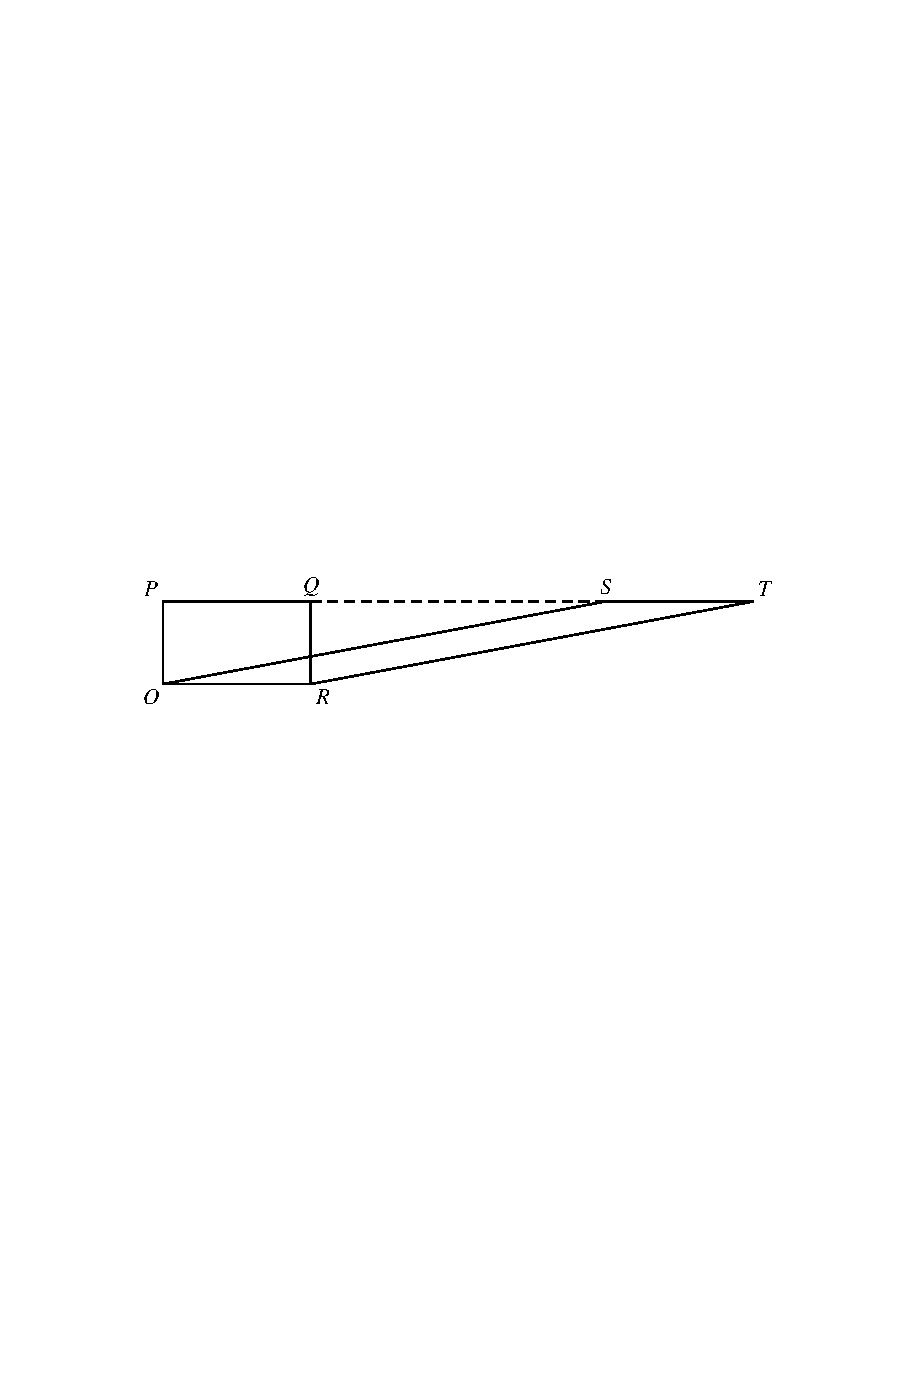
\includegraphics[width=12cm]{BILDER/BildFlaecheParallelogramm2.pdf}}

%% Beweis durch Adition der Flaeche des Dreiecks ORT und Subtraktion
%% der Flaeche des Dreiecks POS

%\centerline{\includegraphics[width=12cm]{BILDER/BildFlaecheParallelogramm3.pdf}}
%\centerline{\includegraphics[width=12cm]{BILDER/BildFlaecheParallelogramm4.pdf}}

Für ein Dreieck folgt entsprechend:
$$
    \mbox{Fläche des Dreiecks} \; = \; \frac{1}{2} \cdot |\mbox{Grundseite}| \cdot |\mbox{Höhe}|
$$

\subsection*{Proportionalitätsprinzip und Anwendungen}

Aus der Formel für die Fläche eines Dreiecks lässt sich ein wichtiges {\em Proportionalitätsprinzip}
ableiten:

%% Das folgende ist Euklid I.37!? bzw. Euklid VI.1

\begin{quote}
    Die Flächen von Dreiecken mit einer gleich langen Grundseite (Höhe) verhalten sich proportional
    zu ihrer Höhe (Grundseite).
\end{quote}

In Euklids Elementen ist die Herleitung dieses Prinzips sehr umständlich, weil ihm ein moderner
Zahlbegriff (insbesondere die reellen Zahlen) fehlten. In Buch V und VI führt er hierfür eine
komplizierte "`Proportionstheorie"' ein.

Interessante Anwendungen des Proportionalitätsprinzips sind einfache Beweise für den Satz des
Pythagoras und für den Strahlensatz. %\ref{thm:strahlensatz}
% Bilder aus Stillwell!! (S.32-33)

%\centerline{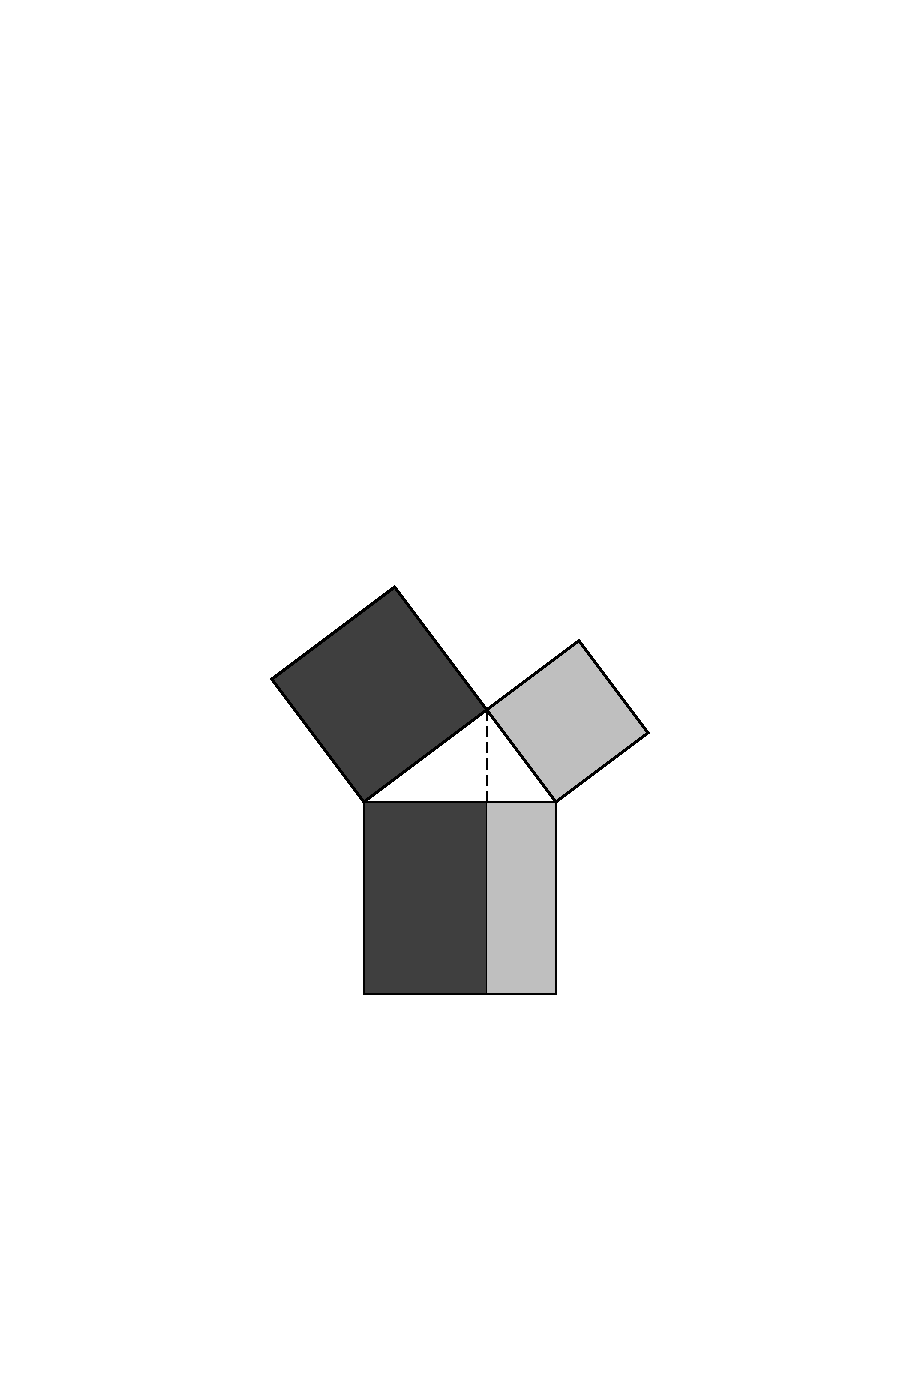
\includegraphics[width=8cm]{BILDER/BildSatzDesPythagoras.pdf}}

\begin{figure}[h]
    \begin{tabular}{cccc}
    \begin{tikzpicture}[line cap=round,line join=round,>=triangle 45,x=1.0cm,y=1.0cm]
        \clip(-1.5,0) rectangle (2,3);
        \draw (0,0) coordinate (A);
        \draw (2,0) coordinate (B);
        \draw (2,2) coordinate (C);
        \draw (0,2) coordinate (D);
        \draw (-0.90,1.43) coordinate (E);
        \draw (-1.48,2.33) coordinate (F);
        \draw (-0.57,2.90) coordinate (G);
        \filldraw [fill=colPktKon] (E)--(G)--(D)--(E);
        \draw (A)--(B)--(C)--(D)--(A)--(E)--(D)--(G)--(F)--(E);
    \end{tikzpicture}
&
    \begin{tikzpicture}[line cap=round,line join=round,>=triangle 45,x=1.0cm,y=1.0cm]
        \clip(-1.5,0) rectangle (2,3);
        \draw (0,0) coordinate (A);
        \draw (2,0) coordinate (B);
        \draw (2,2) coordinate (C);
        \draw (0,2) coordinate (D);
        \draw (-0.90,1.43) coordinate (E);
        \draw (-1.48,2.33) coordinate (F);
        \draw (-0.57,2.90) coordinate (G);
        \filldraw [fill=colPktKon] (A)--(G)--(D)--(A);
        \draw (A)--(B)--(C)--(D)--(A)--(E)--(D)--(G)--(F)--(E);
    \end{tikzpicture}
&
    \begin{tikzpicture}[line cap=round,line join=round,>=triangle 45,x=1.0cm,y=1.0cm]
        \clip(-1.5,0) rectangle (2,3);
        \draw (0,0) coordinate (A);
        \draw (2,0) coordinate (B);
        \draw (2,2) coordinate (C);
        \draw (0,2) coordinate (D);
        \draw (-0.90,1.43) coordinate (E);
        \draw (-1.48,2.33) coordinate (F);
        \draw (-0.57,2.90) coordinate (G);
        \draw [dash pattern=on 4pt off 4pt] (E)--(2,1.43);
        \filldraw [fill=colPktKon] (E)--(D)--(C)--(E);
        \draw (A)--(B)--(C)--(D)--(A)--(E)--(D)--(G)--(F)--(E);
    \end{tikzpicture}
&
    \begin{tikzpicture}[line cap=round,line join=round,>=triangle 45,x=1.0cm,y=1.0cm]
        \clip(-1.5,0) rectangle (2,3);
        \draw (0,0) coordinate (A);
        \draw (2,0) coordinate (B);
        \draw (2,2) coordinate (C);
        \draw (0,2) coordinate (D);
        \draw (-0.90,1.43) coordinate (E);
        \draw (-1.48,2.33) coordinate (F);
        \draw (-0.57,2.90) coordinate (G);
        \draw [dash pattern=on 4pt off 4pt] (E)--(2,1.43);
        \filldraw [fill=colPktKon] (0,1.43)--(D)--(C)--(0,1.43);
        \draw (A)--(B)--(C)--(D)--(A)--(E)--(D)--(G)--(F)--(E);
    \end{tikzpicture}
\end{tabular}

    \caption{Proportionalitätsprinzip am Satz des Pythagoras}
\end{figure}

Der im Bild angedeutete Beweis für den Satz von Pythagoras zeigt in drei Schritten, dass der
Flächeninhalt (bzw. der halbe Flächeninhalt) eines kleinen Quadrats gleich dem Flächeninhalt eines
enstprechenden Rechtecks innerhalb des großen Quadrats ist. Dabei wird im ersten und dritten Schritt
das Proportionalitätsprinzip angewendet und im zweiten Schritt das SWS-Kriterium. Diese Beweisidee
geht auf Euklid zurück.

\begin{proof}[Beweis des Strahlensatzes \ref{thm:strahlensatz}]
    Wir betrachten ein Dreieck $ABC$ und Punkte $P,Q$ wie im Satz angegeben. % siehe Bild...

    \begin{center}
        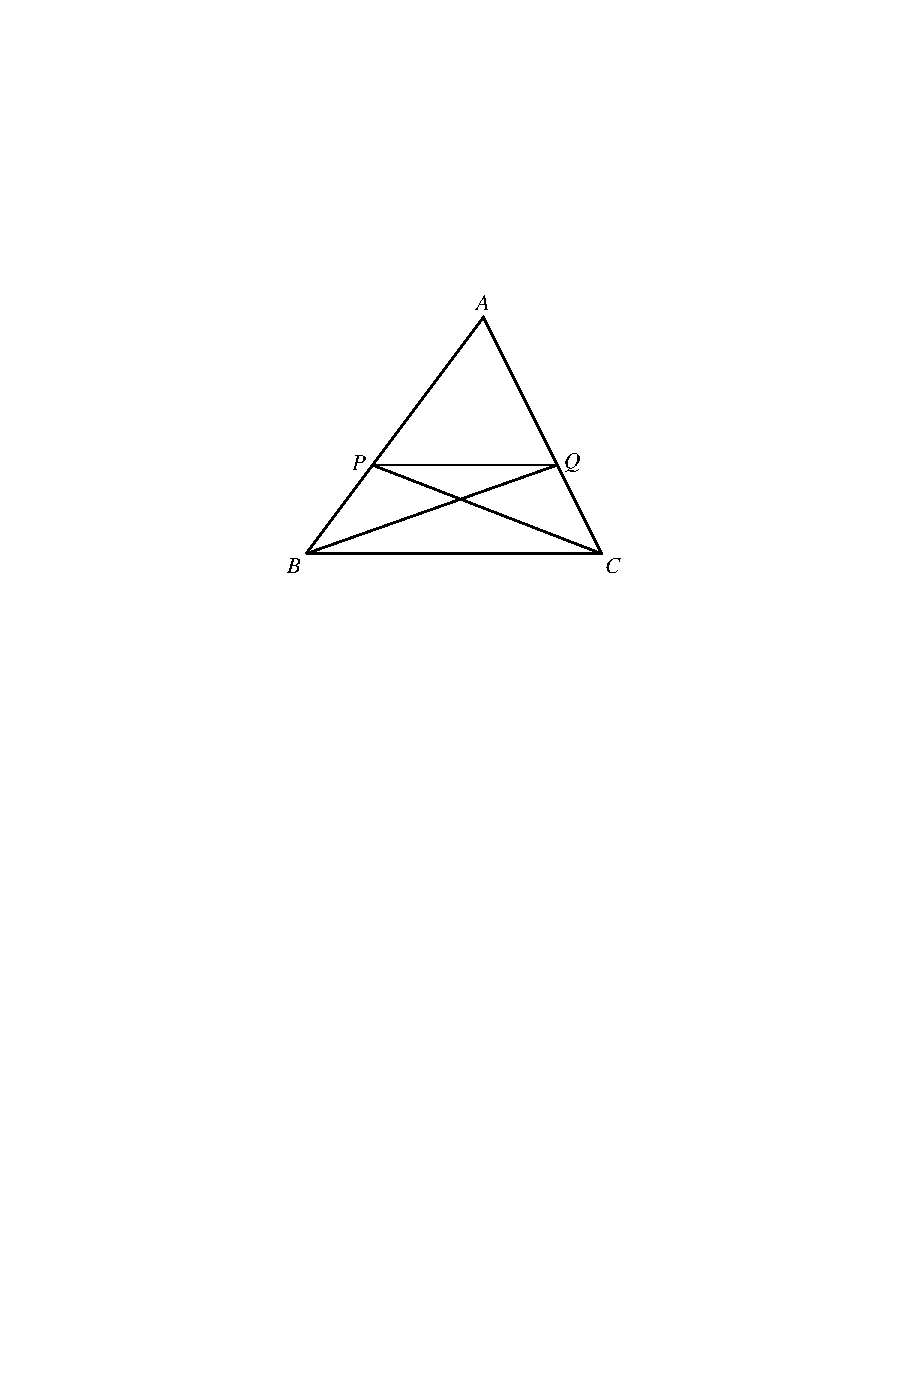
\includegraphics[width=8cm]{BILDER/BildBeweisStrahlensatz.pdf}
    \end{center}

    Weil die Geraden duch $P,Q$ und $B,C$ nach Voraussetzung parallel sind, haben die Dreiecke $PQB$
    und $PQC$ die gleiche Höhe und damit, nach dem Propotionalitätsprinzip, den gleichen
    Flächeninhalt: $|PQB|=|PQC|$. Durch Addition der Fläche des Dreiecks $APQ$ stellen wir fest, das
    die Dreiecke $AQB$ und $APC$ ebenfalls den gleichen Flächeninhalt haben.

    Die Dreiecke $APQ$ und $PQB$ haben die gleiche Höhe in Bezug auf ihre Grundseiten auf der
    Geraden durch $A$ und $B$. D.h., nach dem Propotionalitätsprinzip verhalten sich die Längen der
    Grundseiten zueinander wie ihre Flächeninhalte:
    $$
    \frac{|APQ|}{|AQB|} = \frac{|AP|}{|PQ|}
    $$
    Durch ein analoges Argument für die Dreiecke $PQC$ und $APQ$ erhält man auch
    $$
    \frac{|APQ|}{|PQC|} = \frac{|AQ|}{|QC|}.
    $$
    Wegen $|PQB|=|PQC|$ sind die beiden rechten Seiten gleich, und damit auch die beiden linken
    Seiten.
\end{proof}

{\em Kritik:} Der Beweis des Strahlensatzes verwendet das Proportionalitätsprinzip. Für den Beweis
des Proportionalitätsprinzips benötigt man auch eine Form des Strahlensatzes, so dass es hier in
Euklids Werk zu einem unerlaubten "`Ringschluss "'\ kommt.

% Anmerkung aus Neßelmann-Skript:
%In der Schule wird der Strahlensatz mitunter \"{u}ber Fl\"{a}cheninhalte von
%Dreiecken behandelt, und zwar mit der bekannten Formel
%$F=\frac{1}{2}\cdot g\cdot h$. F\"{u}r den Beweis der Unabh\"{a}ngigkeit der
%Formel von der Auswahl der Grundlinie wird aber gerade der
%Strahlensatz ben\"{o}tigt, wodurch man unwillk\"{u}rlich in einen
%Zirkelschluss ger\"{a}t. Daher f\"{u}hrt dieser Weg zu \underline{keinem}
%Beweis des Strahlensatzes:

%% FOLGENDES AN DEN ANFANG JEDER VORLESUNG (und genauer??)?!?
%\subsection*{Literatur}
%\cite[Kapitel 1 und 2]{SS-2005},
%\cite[Chapter 1]{stillwell-2005},
%\cite[Chapter 1]{hartshorne-2000}
%\cite[Chapter 1]{coxeter-1969}
